% parent style
\documentclass[12pt]{amsart}
\usepackage[margin=0.5in]{geometry}

% Fira Sans, Euler Math, Inconsolata
\usepackage[varg]{txfonts}
\usepackage[T1]{fontenc}
\usepackage[sfdefault]{FiraSans}
\usepackage[small,euler-digits]{eulervm}
\usepackage{textcomp}

% metadata: date and filename
\usepackage[english]{datetime2}
\usepackage{currfile}

% set \today as YYYY-MM-DD

% pandoc is utf8 native
\usepackage[utf8]{inputenc}

% pandoc transfers h2 to subsections, I prefer h2 for sections
\let\subsubsection\subsection
\let\subsection\section
\let\section\chapter
\let\chapter\part

% urls as footnotes
\usepackage[unicode=true]{hyperref}
\renewcommand{\href}[2]{#2\footnote{\url{#1}}}

% formatting
\usepackage{multicol}
\usepackage[dvipsnames]{xcolor}
\usepackage{caption}
\usepackage{fancybox}
\usepackage{graphicx}
\usepackage{float}

\tolerance=1
\emergencystretch=\maxdimen
\hyphenpenalty=10000
\hbadness=10000
\begin{document}

% header
\begin{flushleft}
{\small \color{BurntOrange} \textsc{Departments of Computer Science and Mathematics}}}
\vspace{0.5em}
\end{flushleft}
\begin{center}
{\huge \textbf{\textsc{The Neural Network}}}
\end{center}
\begin{flushright}
{\small \color{BurntOrange} \textsc{Learning about our community}}
\end{flushright}

% footer
\newcommand\blfootnote[1]{%
  \begingroup
  \renewcommand\thefootnote{}\footnote{#1}%
  \addtocounter{footnote}{-1}%
  \endgroup
}
\DTMsetdatestyle{iso}
\blfootnote{
    \textit{Date:} \date\, 
    \textit{Compiled:} \today.
% $if(author)$
% \author{$for(author)$$author$$sep$ \and $endfor$}
% $endif$
% $if(date)$
% \date{$date$}
% $endif$
% $if(repo)$
% $endif$
}
\vspace{-1em}
\begin{multicols}{2}
% photo
\begin{figure}[H]
    \setlength{\fboxsep}{8pt}
    \shadowbox{\parbox{0.45\textwidth}{
    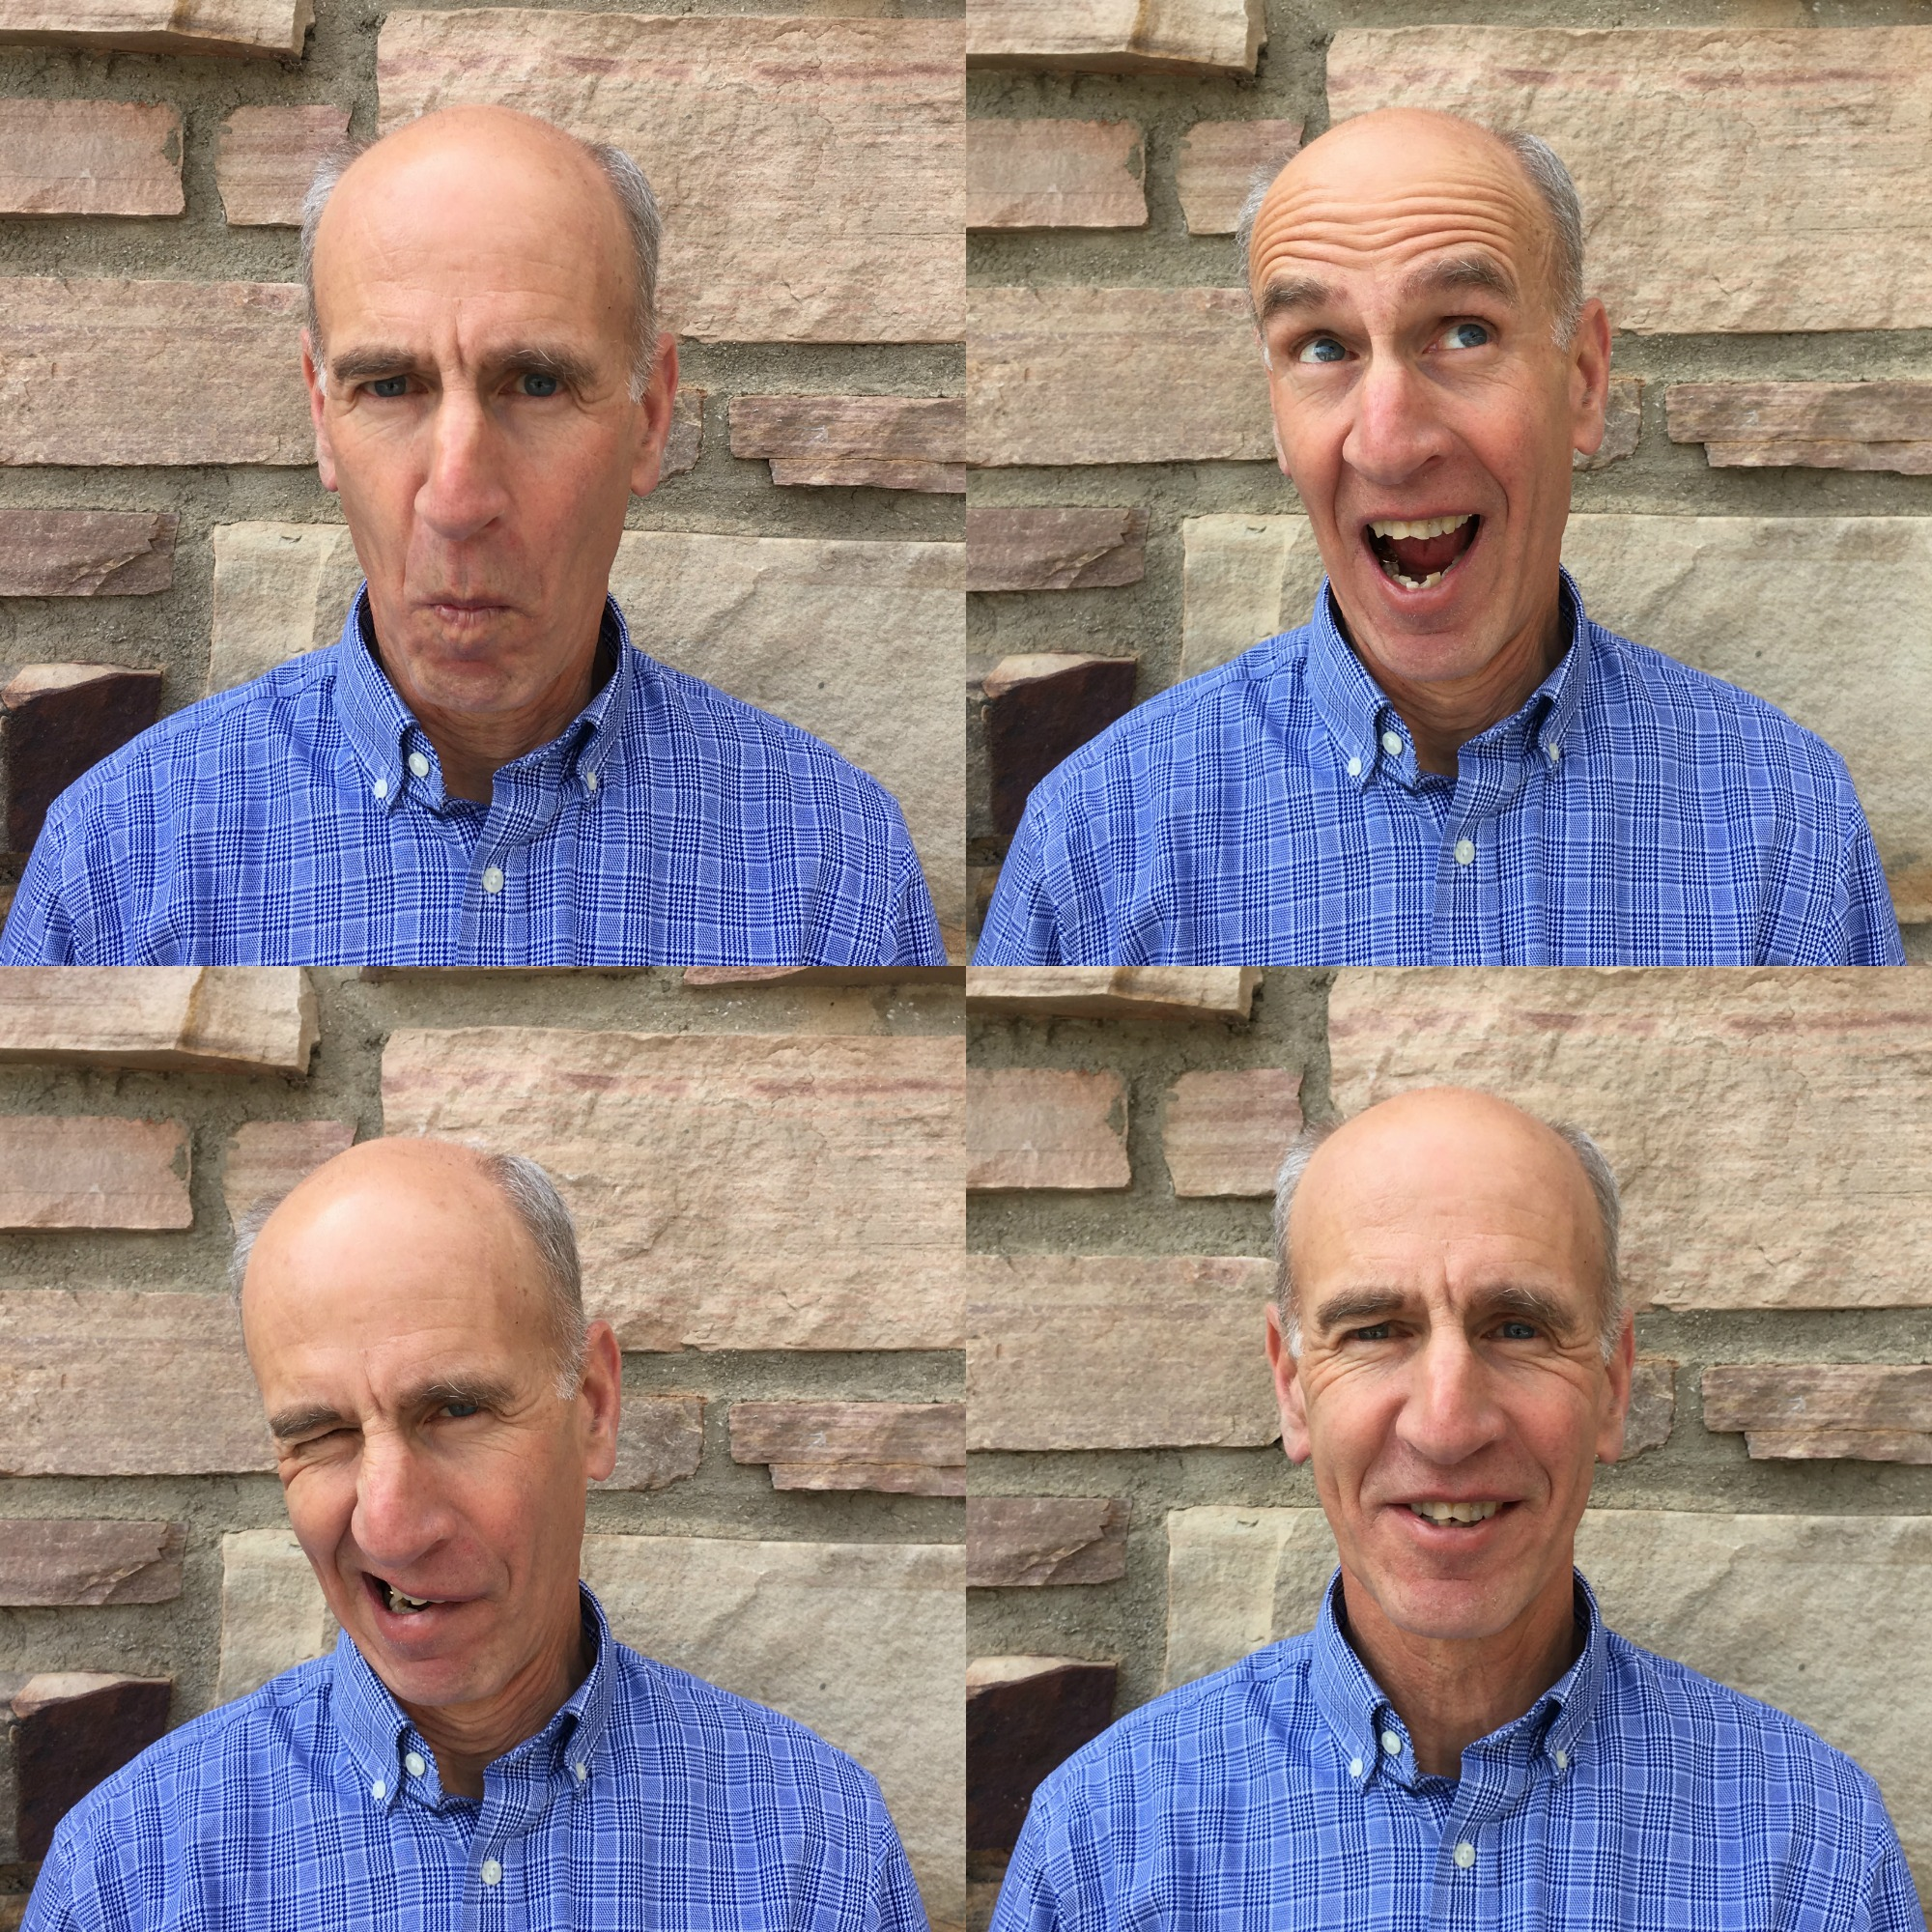
\includegraphics[width=\linewidth]{bobbyschnabel.jpg}
    \caption*{\Large\textbf{\textsc{Bobby Schabel}}}
           }}
\end{figure}
% $if(title)$
% \title{$title$}
% $endif$
% abstract

Given the many titles and roles Bobby Schnabel has held in the
Computer Science department, he is an extremely difficult man to
introduce.  Although he self-identifies as “Chief Maverick and
Rabble Rouser”, Bobby is also the founding director of the ATLAS
Institute, an external chair for the CS department, the co-founder of
the National Center for Women and Information Technology (NCWIT),
the College of Engineering and Applied Science Faculty Director for
Entrepreneurship, and the Campus Thought-Leader on Computing.
Do you see Bobby around campus and want to get to know him
better? He is extremely kind, eager to meet new people, and
wonderful to talk to—just reach out and say hi!


You've had a lot of different roles, what did you learn from each?

Bobby says that he's learned two main lessons from his many 
different experiences. First of all, he's learned the value of working 
with a lot of people with a vision, particularly in academia. 
Furthermore, he's learned the value of listening to and learning 
from people who don't share that vision. Bobby has also learned 
the importance of working with external supporters of an idea: those 
who aren't directly involved in the vision or team, but who are 
involved through fundraising and spreading ideas. Bobby says that at 
the beginning of his career he never would have expected to have 
loved fundraising as much as he does. "Fundraising is about 
getting to hang out with interesting people who you otherwise 
wouldn't get to hang out with!" He has found unexpected joy in 
helping people support a cause they believe in, and how rewarding 
the resulting friendships have been.




What are three improbable facts about you?

Bobby was the student manager of Dartmouth Football’s famous
1970 season. He’s also the first US born person in his immediate
family, with all of his other family members being born in either
Vienna or Germany. Bobby also loves to cook and to create through
cooking. When I asked about the most recent dish he created, he
paused to wonder aloud, “what did we call it?” before happily
describing a delicious concoction he and his wife call Egg Delight.
\end{multicols}

\end{document}
